\documentclass[pre,12pt]{revtex4-1}
\usepackage{epsfig,graphics,amssymb,amsmath,subeqnarray,setspace,graphicx,amsthm,subfigure, mathrsfs,colortbl,color,bm,fancyhdr, tabularx, float}

% Header on each page, with team number and page numbering
\pagestyle{fancy}
\lhead{Team \# 12345} 
\rhead{page \thepage \ of \pageref{LastPage}}
\cfoot{}
\renewcommand{\headrulewidth}{0.4pt}
\renewcommand{\footrulewidth}{0.0pt}

% Make life easier: define some shortcuts!
\def\b{\bm}
\def\e{\epsilon}
\def\ep{\varepsilon}
\def\u{\underline}
\def\c{\centerline}
\def\n{\noindent}
\def\h{\hangindent}


\newcommand{\tcb}{\textcolor{blue}}

% Double spacing is 2, 1.5 spacing is 1.5, ...
\def\baselinestretch{1.0}

% For tables:
\definecolor{Gray}{gray}{0.9}
\newcolumntype{C}{c<{\kern\tabcolsep}@{}}

\begin{document}

\title{Centroids, Clusters, and Crime: Anchoring the Geographic Profiles of Serial Criminals \\(\textbf{Catchy, but informative title})}
\author{Team \# 12345}
\date{\today}

\begin{abstract}
A particularly challenging problem in crime prediction is modeling the behavior of a serial killer. Since finding associations between the victims is difficult, we predict where the criminal will strike next, instead of whom. Such predicting of a criminal's spatial patterns is called geographic profiling.

Research shows that most violent serial criminals tend to commit crimes in a radial band around a central point: home, workplace, or other area of significance to the criminal's activities (for example, a part of town where prostitutes abound). These ``anchor points'' provide the basis for our model.

We assume that the entire domain of analysis is a potential crime spot, movement of the criminal is uninhibited, and the area in question is large enough to contain all possible strike points. We consider the domain a metric space on which predictive algorithms create spatial likelihoods. Additionally, we assume that the offender is a violent serial criminal, since research suggests that serial burglars and arsonists are less likely to follow spatial patterns.

There are substantial differences between one anchor point and several. We treat the single-anchor-point case first, taking the spatial coordinates of the criminal's last strikes and the sequence of the crimes as inputs. Estimating the point to be the centroid of the previous crimes, we generate a ``likelihood crater,'' where height corresponds to the likelihood of a future crime at that location. For the multiple-anchor-point case, we use a cluster-finding and sorting method: We identify groupings in the data and build a likelihood crater around the centroid of each. Each cluster is given weight according to recency and number of points. We test single point vs. multiple points by using the previous crimes to predict the most recent one and comparing with its actual location.
We extract seven datasets from published research. We use four of the datasets in developing our model and examining its response to changes in sequence, geographic concentration, and total number of points. Then we evaluate our models by running blind on the remaining three datasets.
The results show a clear superiority for multiple anchor points.

\textbf{This is the most important section of the paper. Make it beautiful.} The above was the summary page of a winning entry by Damle, West, and Benzel at CU-Boulder in 2010.
\end{abstract}
\maketitle

\newpage

\section{Assumptions}
\begin{itemize}
    \item The water level of Lake Ontario ranges from 74.0 m to 76.0 m. 
    \item Boating season is from April to November.
    \item Environmental conditions are the same for all five lakes.
    \item The efficiency of hydro-power stations is $90$ percent.
    \item Organism within the same class share the same living conditions. 
\end{itemize}

\section{Model 2: Interests Analysis for stakeholders}\label{Model}
\subsection{Technique}
We consider five kinds of stakeholders that are susceptible to the change in the water levels in the Great Lakes area with special attention to Lake Ontario. They are property owners, recreational boaters, hydro-power stations, shipping companies, and environmentalists. In order to predict the optimal water levels across the year, we convert their demands into numerous linear relations and use simplex method to solve the following linear program: \\ 
\begin{align}
    max\quad z = \sum_{i}{f_{i}x} \\
    s.t. \quad Ax \leq b \\
    x \geq 74 \\
    x \leq 76
\end{align}
Where $z$ represents the objective function of this model, which is the weighted sum of normalized economic interests of all stakeholders, $x$ is a vector which represents water level, $A$ is a matrix that contains all the linear constraints that we take into consideration, and $b$ is a vector that encodes thresholds for all constraints. The last two constraints are relaxation of the actual water level range of Lake Ontario. Simplex method starts from a basic solution, which is a vertex of the polyhedron formed by the collection of constraints; then the algorithm travels along edges of the feasible region in a direction that maximizes the objective function until it arrives at the optimal vertex, which is called the basic feasible solution, $i.e.$, the optimal water level. \par
During the research, we realize that the magnitude of data varies from stakeholder to stakeholder. Therefore, we bring all the numbers to the same level by dividing both sides of linear equations with appropriate constants. This step is called normalization. When tuning our model, we gradually discover the relative importance of each stakeholder in our model by temporarily zeroing out its peers in the objective function. The approximate relationship between stakeholders and their weights is shown in Table I. Unfortunately, environmental elements have to subordinate to other activities that have a more direct and significant impact on economy, such as commercial navigation and electricity generation. \\
\begin{table}[H]
\begin{center}
\begin{tabular}{llllll}
\hline
\multicolumn{1}{l|}{Stakeholders} & \multicolumn{1}{l|}{Property}  & \multicolumn{1}{l|}{Hydro-power}  & \multicolumn{1}{l|}{Shipping}   & \multicolumn{1}{l|}{Boaters} & \multicolumn{1}{l}{Environmentalists}  \\ \hline
\multicolumn{1}{l|}{Weights} & \multicolumn{1}{l|}{0.2} & \multicolumn{1}{l|}{0.3} & \multicolumn{1}{l|}{0.3} & \multicolumn{1}{l|}{0.1} & \multicolumn{1}{l}{0.1} \\ \hline
\end{tabular}
\caption{\label{stakeholders & weights}Stakeholders and their weights}
\end{center}
\end{table}


\subsection{Property Owners}
Flooding has always been a major concern for residents and property holders near the lake areas. From \textit{Great Lakes Flood Thresholds and Impacts} (Gabriel et al., 1997), we can find the flood damage thresholds for all five Great Lakes (Figure 1).  \par
\begin{figure}[htbp]
\begin{center}
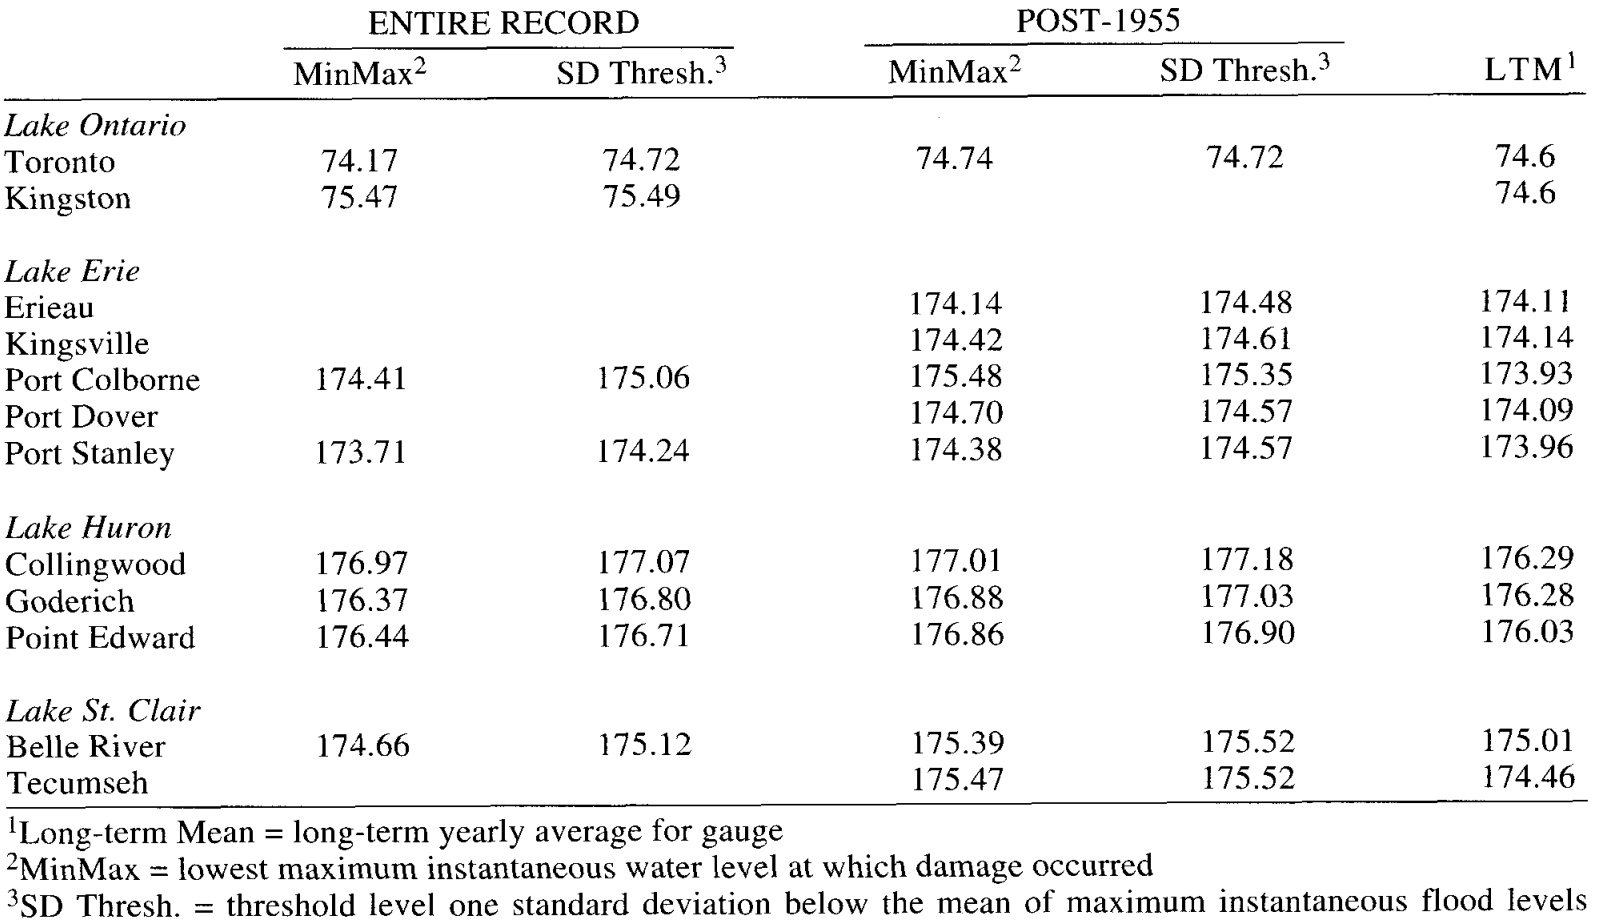
\includegraphics[width=4.5in]{flood.png}
\caption{Summary table of flood damage thresholds by lake and water level gauge. From Ref.~\cite{nd97}.}
\label{leaf}
\end{center}
\end{figure}
Then we consider how much money flooding can cost. According to media, severe flooding triggered by high water level usually makes "soaked" neighborhoods spend several million dollars. Inspired by the paper, we divide the potential flooding of a lake into three levels based on the water surface height of the lake, and consider the frequencies of each level (Figure 2). 
\begin{figure}[htbp]
\begin{center}
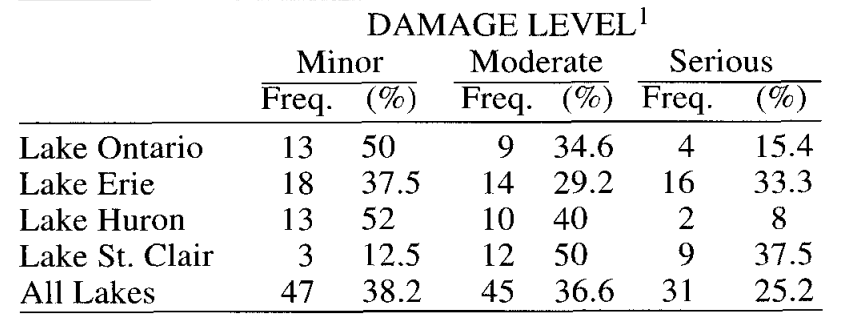
\includegraphics[width=4.5in]{floodfreq.png}
\caption{Summary of flood frequencies and flood thresholds by lake. From Ref.~\cite{nd97}.}
\label{leaf}
\end{center}
\end{figure}
We then associate these different levels of catastrophes with the economic damage caused by them. For the linearity of the model, we keep the cost increasing in a linear way when the water level exceeds a certain threshold. Eventually, we take the negative value of the combined result of these functions and fit it into the objective function we are trying to maximize.

\subsection{Hydro-power Stations}
The Moses-Saunders Power Dam is the major source of hydro-power at Lake Ontario. It supports two hydroelectric power generating stations in that region. A hydro-power station transforms the gravitational potential energy into electricity. With the aim of estimating the power generated by the dam, we quote a formula in physics. 
\begin{align}
    P = \eta Qgh
\end{align}
$P$ is the electric power generated, $Q$ is the discharge of water in $kg/s$, $g$ is the acceleration due to gravity, $h$ is the height of water level, and $\eta$ stands for the efficiency of this process. The ability of generating power is considered as the interest of hydro-power stations and is thus included in the objective function. And we later design a mechanism to control the amount of water discharged at the dam.

\subsection{Recreational Boaters}
Water levels have a large impact on the economy generated by boating. Based on an analysis of this issue performed by Cornell University (Connelly et al., 2005), we first estimate the loss of total possible boating days of each possible water level, correspondingly. Then we use several sets of linear functions to deduce the consequential economical impacts on boating for each month in the boating season. Figure 3 shows this correlation. \par
\begin{figure}[htbp]
\begin{center}
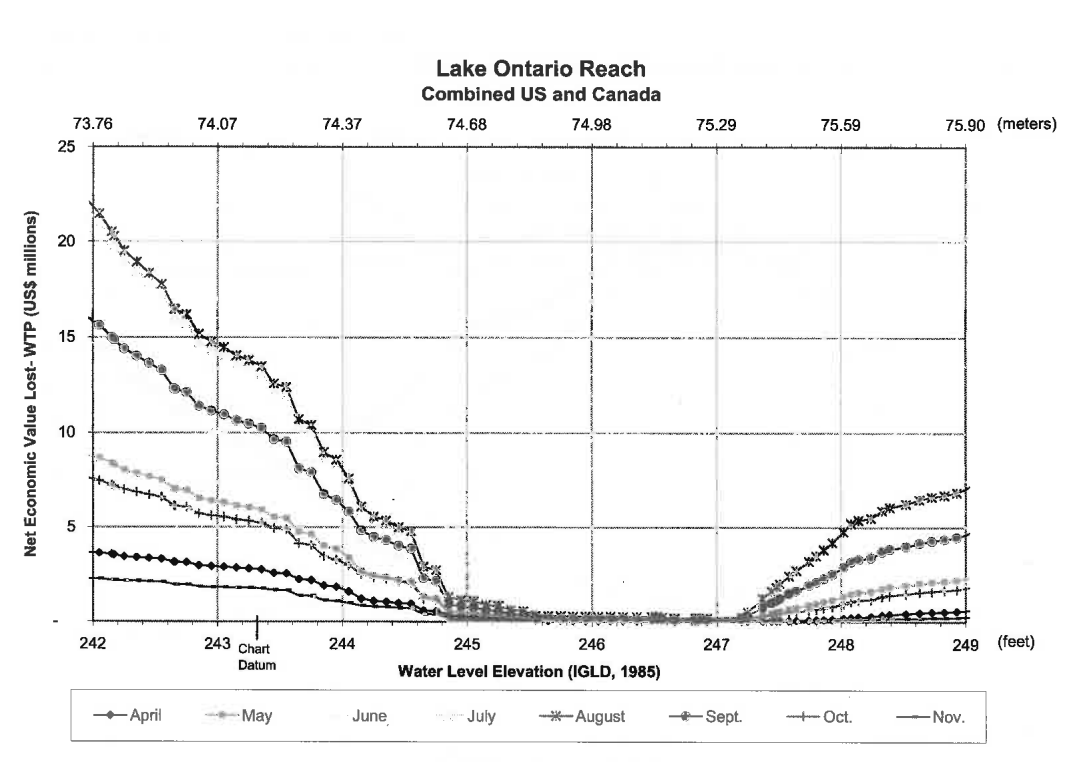
\includegraphics[width=4.5in]{boating.png}
\caption{Relationship between water level and net economic value lost.  From Ref.~\cite{nd05}.}
\label{leaf}
\end{center}
\end{figure}
Using the economic data from the same paper, we consider the inflation rate over the past two decades to obtain a reasonable dataset which contains the economic value of boating in the current market. We also applied a more recent boating preference graph of Lake Ontario from Plan 2014 (Figure 4) to our model. 

\begin{figure}[H]
\begin{center}
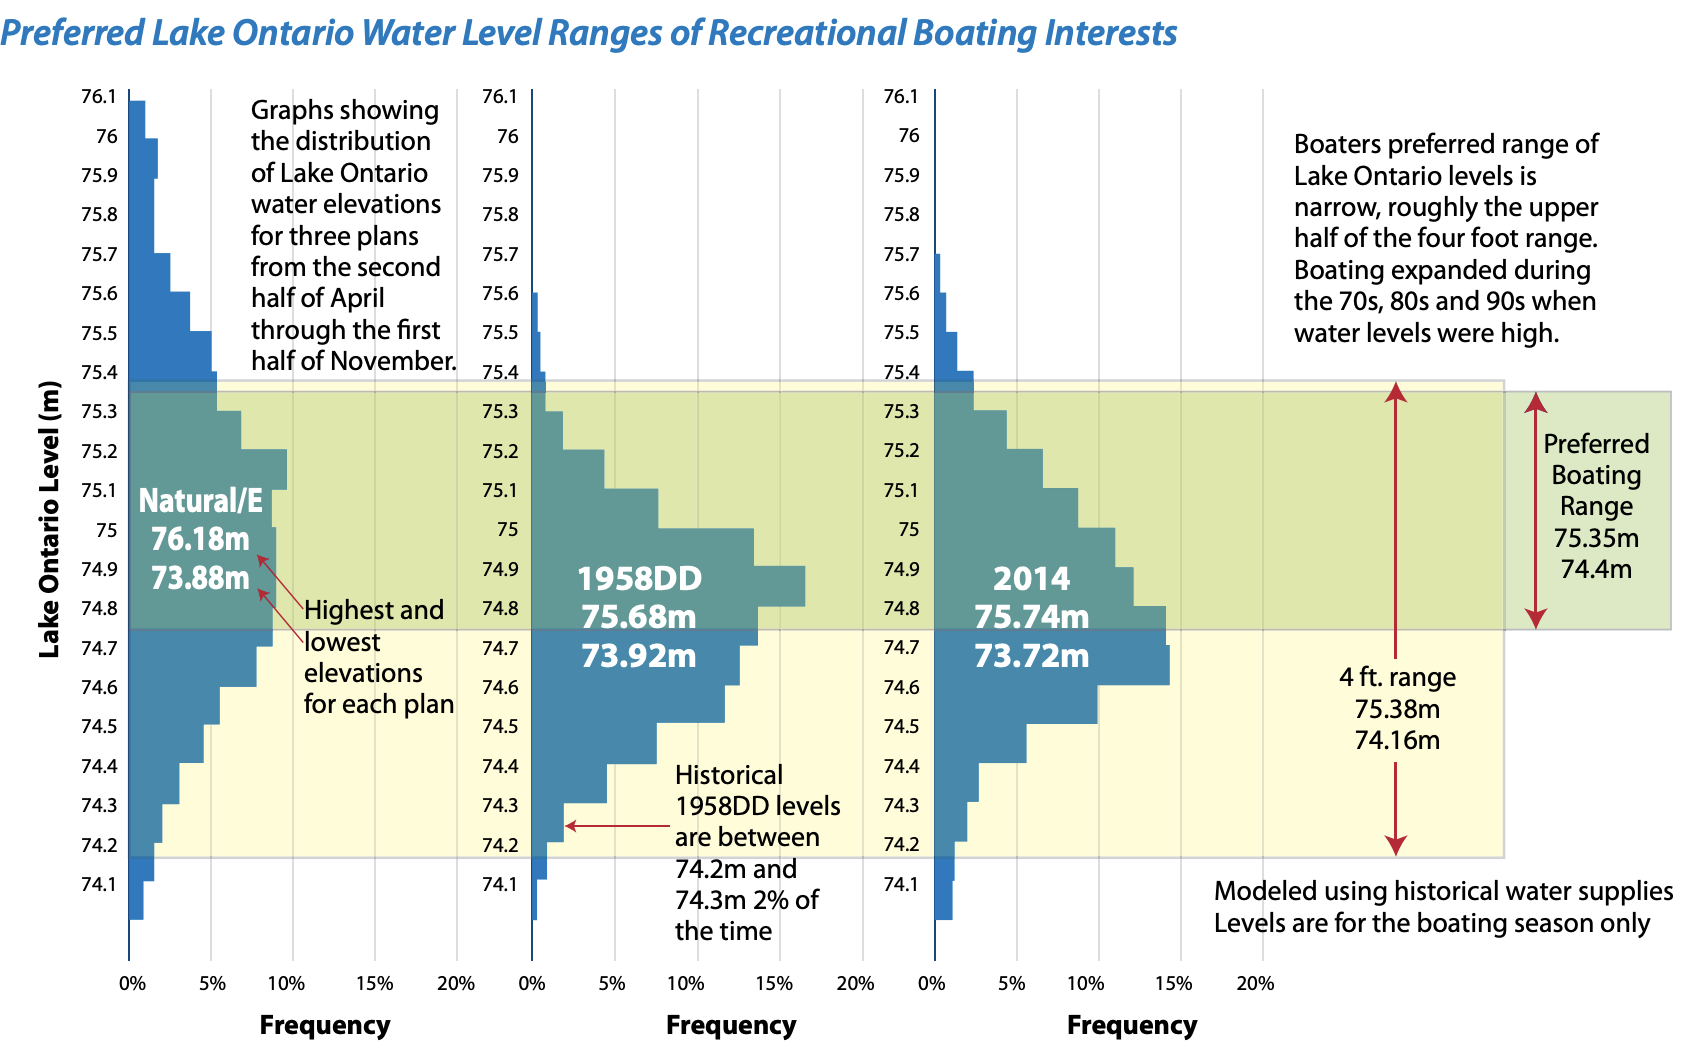
\includegraphics[width=4.5in]{boating2.png}
\caption{Preferred boating range: 74.4m to 75.35m.  From Ref.~\cite{nd14}.}
\label{leaf}
\end{center}
\end{figure}

After that, to make our simplex solver capable of processing the information, we fit a piece-wise linear function by breaking the dataset into segments. For each segment, we use the following method to calculate its slope $m$ and shift $b$:
\begin{align}
    m = \frac{y_{2} - y_{1}}{x_{2} - x_{1}}\\
    b = y_{1} - m \cdot x_{1}
\end{align}
The piece-wise linear function is later used a part of the objective function in our linear programming formulation.

\subsection{Shipping Companies}
Shipping is a vital industry across the Great Lakes, as it boosts GDP, creates enormous job positions, and supports navigation. Ships all prefer steady and high water, so that they can carry more cargo safely. We examine a paper titled \textit{The impact of water level changes on commercial navigation in the Great Lakes and St. Lawrence River}; in this paper, Millerd mentioned that reducing lake level would increase annual shipping costs by 15 to 33 percent (Millerd, 1996). An earlier study demonstrates the economic effects on commercial navigation caused by several regulatory plans on Lake Erie (International Lake Erie Regulation Study Board 1981), Figure 5 shows the major one of them. \par
\begin{figure}[H]
\begin{center}
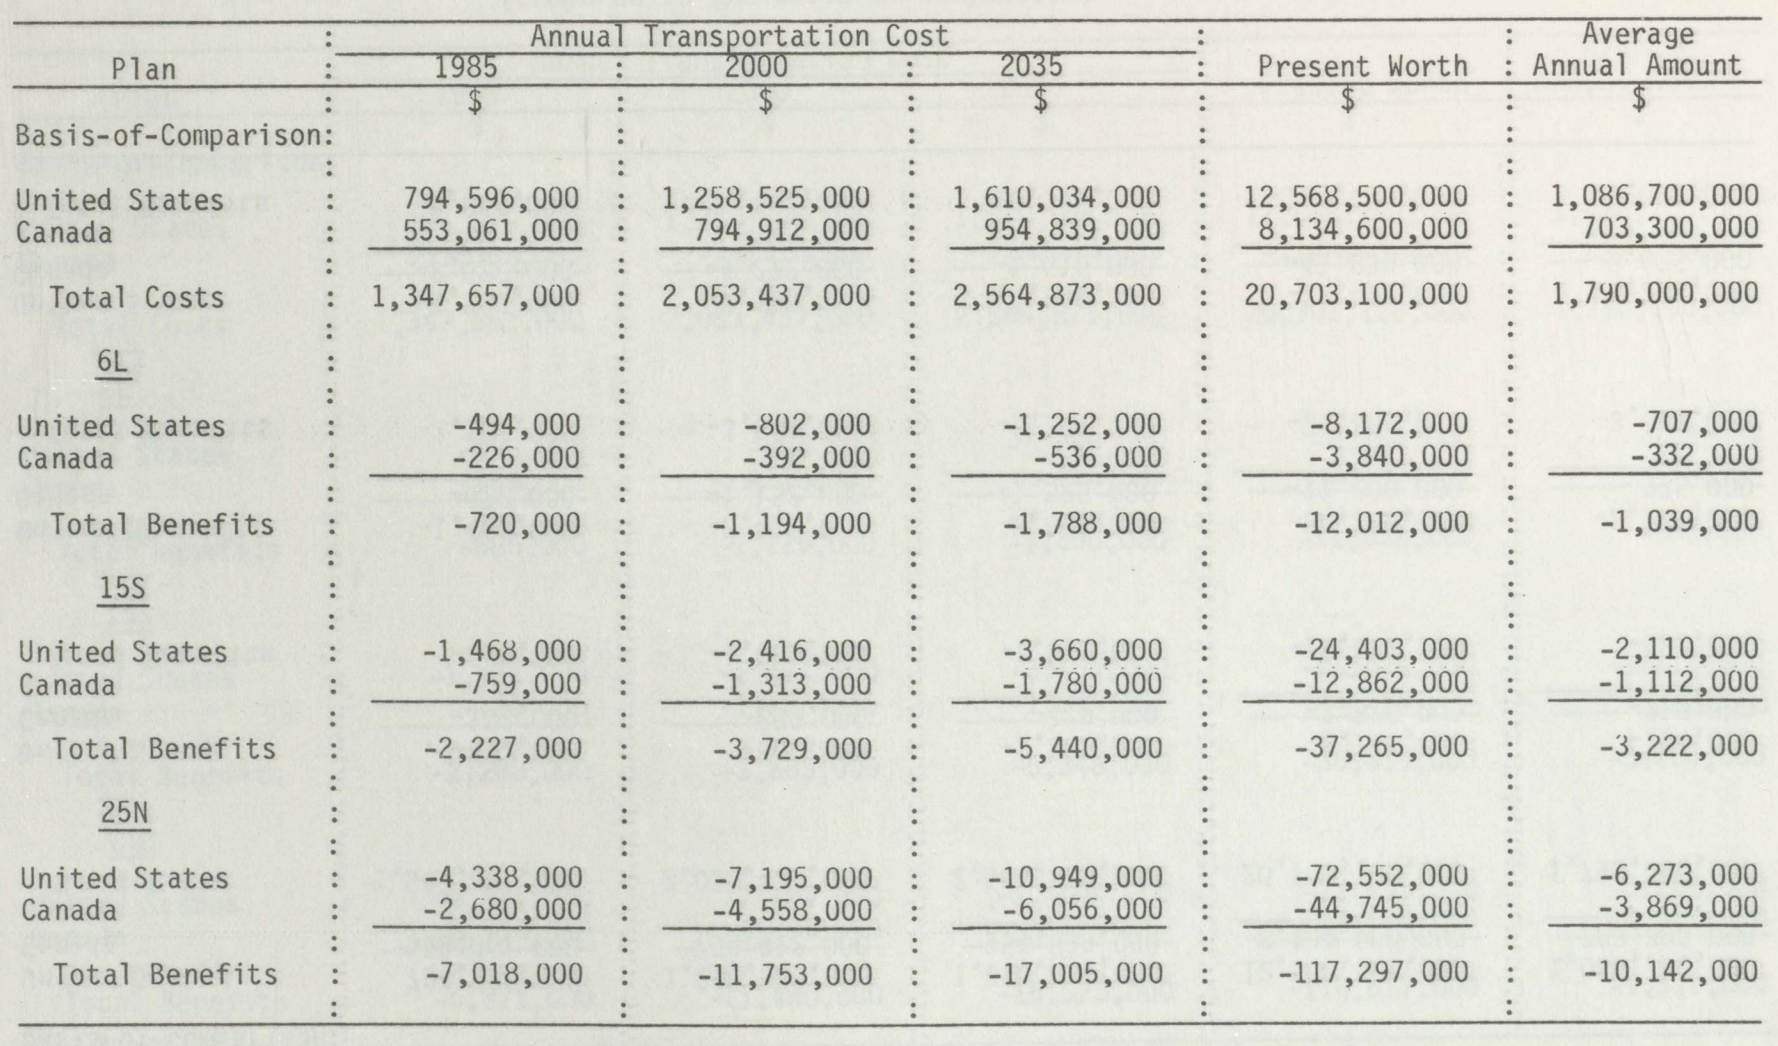
\includegraphics[width=4.5in]{shipping.png}
\caption{Economical impacts on commercial shipping under category 1 of the regulation. From Ref.~\cite{nd81}.}
\label{leaf}
\end{center}
\end{figure}
We develop linear equations that calculate the benefits of commercial navigation based on the data provided in study board and by applying the line-fitting technique we use for boaters. Finally, the economic contribution from shipping is added to the objective function.

\subsection{Environmentalists}
The Great Lakes Basin is the home for more than 3,500 species; the diversity of this huge ecosystem makes environmentalists join the team of stakeholders. Since our goal is to predict the optimal water level, we will focus on wildlife that inhabits in those lakes and the wetlands around the lakes.\par
In the ecosystem assessment of Lake Ontario (Bain et al., 2008), authors utilize a set of impact assessment tools to discuss how the ecosystem of Lake Ontario will be affected subject to water management policies. They analyze reactions from plants, invertebrates, fish, and birds toward the change in water levels. As suggested in their report, an increase that is greater than 1 m can lead to a recession in the nesting suitability of bank swallows; a seasonal change of 0.1 m will alter the available area for floating-leaved aquatic vegetation (Bain et al., 2008)... With gathered information from this paper, we set up linear equations to simulate the effects on the area of available habitats triggered by altering water levels in different months of a year. With the idea of being eco-friendly, creatures' living space is also considered as a component of our objective function.

\begin{thebibliography}{10}
\bibitem{nd97}Anthony, Reid, and Christian. ``Great Lakes Flood Thresholds and Impacts'' Journal of Great Lakes Research 23.3 (1997): 290.

\bibitem{nd05}Nancy, Jean-Francois, Jonathan, and Timothy. ``Estimating the Economic Impact of Changing Water Levels on Lake Ontario and the St. Lawrence River for Recreational Boaters and Associated Businesses'' HDRU Series 05.2 (2005): 7.
\bibitem{nd14} International Joint Commission (2014). Lake Ontario St. Lawrence River Plan 201: Protecting against
extreme water levels, restoring wetlands and preparing for climate change. 

\bibitem{nd81} International Lake Erie Regulation Study Board (1981). Lake Erie Water Level Study: Lake Erie Regulation Study. Report by the International Lake Erie Regulation Study Board: Appendix G. Recreational Beaches and Boating. International Joint Commission (IJC) Digital Archive. https://scholar.uwindsor.ca/ijcarchive/275

\bibitem{nd08}Bain, M. B., Singkran, N., and Mills, K. E. (2008). Integrated ecosystem assessment: Lake Ontario water management. PloS one, 3(11), e3806. https://doi.org/10.1371/journal.pone.0003806
\end{thebibliography}
\end{document}

